%---------- Inleiding ---------------------------------------------------------

\section{Introductie}%
\label{sec:introductie}

% Met een jaarlijks budget van 32 miljoen in het vakgebied kunstmatige intelligentie (AI) op de werkvloer is België een pionier \autocite{Crevits2022}.  Zo zijn er verschillende projecten, om taalgerelateerde AI-ontwikkelingen op te starten, uit de grond gestampt. Het amai!-project \footnote{https://amai.vlaanderen/}  verenigt AI-softwarebedrijven uit verschillende domeinen om zo met AI-toepassingen te maken die processen automatiseren om de werkdruk te verminderen, zoals binnen het onderwijs \textit{real-time} ondertiteling en een taalassistent voor leerkrachten in meertalige klasgroepen.

Het middelbaar onderwijs staat op barsten. De aanhoudende werkdruk voor leerkrachten en scholieren loopt gelijk met de neergaande kwaliteit van het Vlaamse middelbare onderwijs. Het STEM-agenda\footnote{https://www.vlaanderen.be/publicaties/stem-agenda-2030-stem-competenties-voor-een-toekomst-en-missiegericht-beleid} van de Vlaamse Overheid bestaat uit aandachtspunten om het STEM-onderwijs tegen 2030 aantrekkelijker te maken door de ondersteuning voor zowel leerkrachten als scholieren te verbeteren. De werkdruk bij leraren en scholieren in het middelbaar onderwijs ligt torenhoog. STEM heeft een prominente rol binnen het onderwijs gekregen. De derde graad van het middelbaar onderwijs is een cruciale stap voor de verdere loopbaan van scholieren. Het overbruggen van wetenschappelijke jargon is echter nergens in de aandachtspunten terug te vinden, maar tekstvereenvoudiging met kunstmatige intelligentie biedt hier een revolutionaire oplossing aan.

Dit onderzoek wijst uit hoe de inhoud van een wetenschappelijk artikel met kunstmatige intelligentie vereenvoudigd kan worden, gericht op de noden van scholieren met dyslexie in de derde graad middelbaar onderwijs. Eerst haalt het onderzoek aan wat tekstvereenvoudiging is en hoe een wetenschappelijk artikel vereenvoudigd kan worden. Daarna wijst het onderzoek uit hoe tekstvereenvoudiging met AI scholieren met dyslexie van het derde graad middelbaar onderwijs kan helpen. Nadien staat het onderzoek stil bij de struikelblokken op taalvlak waarmee een toepassing rekening mee moet houden. Als volgt haalt het onderzoek aan welke bestaande toepassingen en \textit{proof-of-concepts} teksten vereenvoudigen. Deze fase omvat ook een zelfgemaakte pipeline voor tekstvereenvoudiging. Ten slotte haalt het onderzoek de verschillende evaluatietechnieken aan die nodig zijn om een vereenvoudigde tekst te beoordelen, alsook welke ethische aspecten ontwikkelaars in acht moeten houden bij het opzetten van een dergelijke toepassing. Het onderzoek eindigt met een vergelijkende studie van de aangehaalde toepassingen, waarbij de vereenvoudigde tekstinhoud aan de hand van \textit{surveys} en statistische metrieken wordt beoordeeld.

%---------- Stand van zaken ---------------------------------------------------

\section{State-of-the-art}%
\label{sec:state-of-the-art}

% De sprong in AI gaf wereldwijd de aanzet om taalgerelateerde AI-toepassingen te ontwikkelen. ChatGPT\footnote{https://chat.openai.com/chat} van OpenAI is een chatbot met onder andere een simplificatiefunctie dat nu werkt op GPT-3, een API tegen aanbetaling. Nadelig moet de chatbot expliciet gevraagd worden om een bepaalde actie mogelijk te maken. Readable\footnote{https://readable.com/} is een online Engelstalige tool dat zinnen beoordeeld op basis van leesbaarheidsformules. Bij beide tools is het enkel mogelijk om tekst op de webpagina te plakken, dus er kunnen geen PDF-documenten of scans worden geüpload en eenzelfde werking verwachten. Op Nederlands vlak zijn er online verschillende samenvattingstools beschikbaar. Enkele voorbeelden zijn: Resoomer\footnote{https://resoomer.com/nl/}, Paraphraser\footnote{https://www.paraphraser.io/nl/tekst-samenvatting} en Prepostseo\footnote{https://www.prepostseo.com/tool/nl/text-summarizer}.

% Deelvraag: Wat is tekstsimplificatie
De voorbije tien jaar is kunstmatige intelligentie (AI) sterk verder ontwikkeld. De toename in kennis zorgde voor nieuwe toepassingen. Tekstvereenvoudiging vloeide hier uit voort. Momenteel bestaan er al robuuste toepassingen die teksten kunnen vereenvoudigen, zoals Resoomer\footnote{https://resoomer.com/nl/}, Paraphraser\footnote{https://www.paraphraser.io/nl/tekst-samenvatting} en Prepostseo\footnote{https://www.prepostseo.com/tool/nl/text-summarizer}. Binnen het kader van tekstvereenvoudiging is er bestaande documentatie beschikbaar waar onderzoekers het voordeel van toegankelijkheid aanhalen, maar deze toepassingen ontbreken de extra noden die scholieren met dyslexie in het derde graad middelbaar onderwijs vereisen.

Het algemene doel van tekstvereenvoudiging is om ingewikkelde bronnen toegankelijker te maken. Het zorgt voor verkorte teksten zonder de kernboodschap te verliezen. Tekstvereenvoudiging gebeurt doorgaans op één van drie manieren. Er is conceptuele vereenvoudiging waarbij documenten naar een compacter formaat worden getransformeerd. Daarnaast is er uitgebreide modificatie die kernwoorden aanduidt door gebruik van redundantie. Als laatste is er samenvatting die documenten verandert in kortere teksten met alleen de topische zinnen. Met deze concepten zijn ontwikkelaars in staat om ingewikkelde woorden te vervangen door eenvoudigere synoniemen of zinnen te verkorten zodat ze sneller leesbaar zijn \autocite{Siddharthan2014}.

Tekstvereenvoudiging behoort tot de zijtak van natuurlijke taalverwerking (NLP) in kunstmatige intelligentie. NLP omvat methodes om, door machinaal leren, menselijke teksten om te zetten in tekst voor machines. Documenten vereenvoudigen met NLP kan op twee manieren: extract of abstract. Bij extractieve simplificatie worden zinnen gelezen zoals ze zijn neergeschreven. Vervolgens bewaart een document de belangrijkste taalelementen om de tekst te kunnen hervormen. Deze vorm van tekstvereenvoudiging komt het meeste voor \autocite{Sciforce2020}. Daarnaast is er abstracte simplificatie die de kernboodschap van de zin bewaart en daarmee een nieuwe zin opbouwt. Volgens het onderzoek van \textcite{Chowdhary2020} heeft deze vorm potentieel dankzij de menselijke interpretatie, maar zit nog in de kinderschoenen.

% Deelvraag 2: Bewezen voordelen van tekstsimplificatie bij scholieren met dyslexie
Voor kinderen met dyslexie bestaan digitale hulpmiddelen die voor een betere visuele presentatie zorgen van teksten. Zo haalt het onderzoek van \textcite{Rello2012} tips aan waarmee teksten en documenten rekening moeten houden bij scholieren met dyslexie in het derde graad middelbaar onderwijs. Het gaat over speciale lettertypes, spreiding tussen woorden en het gebruik van inzoomen op aparte zinnen. Het onderzoek haalt aan dat teksten voor deze unieke noden aanpassen tijdrovend is, dus tekstvereenvoudiging door kunstmatige intelligentie kan een revolutionaire oplossing bieden. 

Het onderzoek van Franse wetenschappers \newline \textcite{Gala2016} illustreert dat manuele tekstvereenvoudiging schoolteksten toegankelijker \newline maakt voor kinderen met dyslexie. Dit deden ze door simpelere synoniemen en zinsstructuren te gebruiken. Verwijswoorden werden vermeden en woorden kort gehouden. De resultaten waren veelbelovend. Het leestempo lag hoger en de kinderen maakten minder leesfouten. Ook bleek er geen verlies van begrip in de tekst bij geteste kinderen. Resultaten van de studie werden gebundeld voor de mogelijke ontwikkeling van een AI-hulpmiddel.

De Universiteit van Kopenhagen is met bovenstaande idee aan de slag gegaan. Onderzoekers \textcite{Bingel2018} hebben gratis software ontwikkeld, genaamd Hero\footnote{https://beta.heroapp.ai/}, om tekstvereenvoudiging voor scholieren in het middelbaar onderwijs met dyslexie te automatiseren. De software bestudeert met welke woorden de gebruiker moeite heeft, en vervangt die door simpelere alternatieven. Hero bevindt zich in beta-vorm en wordt enkel in het Engels en het Deens ondersteund. 

% Deelvraag: Waarop moet er gefixeerd worden bij een wetenschappelijke paper
\textcite{PlavenSigray2017} halen aan hoe onderzoekers in hun taalbubbel blijven, wat gevolgen voor de lezers met zich meebrengt. Daarnaast brengt de stijging aan het gebruik van acroniemen volgens \textcite{Barnett2020} een extra obstakel met zich mee. Het onderzoek van \textcite{Donato2022} wijst erop dat ondoorgrondelijke teksten te wijten zijn aan scholieren met dyslexie in het middelbaar onderwijs die uit hun richting vallen, wat voornamelijk bij STEM-richtingen het geval is. 

% Deelvraag: Uitdagingen van AI-software met tekstsimplificatie
NLP is de laatste decennia volop in ontwikkeling, maar ontwikkelaars botsen nog op uitdagingen. Het gaat om zowel interpretatie- als dataproblemen bij AI-machines. Allereerst is het voor een machine moeilijk om de context van homoniemen te achterhalen. Bijvoorbeeld bij het woord ‘bank’ is het niet duidelijk voor de machine of het gaat over de geldinstelling of het meubel. Daarnaast zijn synoniemen geen probleem voor tekstverwerking \autocite{Roldos2020}.

Het merendeel van NLP-toepassingen maakt gebruik van Engelstalige invoer. Niet-Engelstalige toepassingen zijn zeldzaam. De opkomst van AI-technologieën die twee datasets gebruiken, biedt een oplossing voor dit probleem. De software vertaalt eerst de oorspronkelijke tekst naar de gewenste taal, voordat de tekst wordt herwerkt \autocite{Sciforce2020}. Hetzelfde onderzoek bewijst dat het vertalen van gelijkaardige talen, zoals Duits en Nederlands, een minimaal verschil opleverd.

% Deelvraag: Stand van zaken bij Belgische secundaire scholen
De Vlaamse overheid leent gratis abonnementen uit voor voorlees- en schrijfsoftware. De voornaamste zijn SprintPlus\footnote{https://www.sprintplus.be/}, Alinea\footnote{https://sensotec.be/product/alinea-suite/} en Kurzweil3000\footnote{https://sensotec.be/product/kurzweil-3000/}. Vlaamse scholieren met dyslexie in het middelbaar onderwijs kunnen voor deze software een gratis abonnement of licentie aanvragen. Al bieden de vijf softwarepaketten elk een eigen samenvattingsfunctie, de focus ligt echter op spreek- en luistersoftware waarbij het samenvatten en markeren van tekst als extra wordt gehouden.

ChatGPT\footnote{https://chat.openai.com/chat} van OpenAI is een opkomend chatbot gebouwd op het GPT-3 model. Het GPT-3 model omvat meer dan vijf miljard verschillende woorden, wat het revolutionair maakt voor AI-taaltoepassingen. Nadelig moet de chatbot via de online toepassing expliciet gevraagd worden om tekst te kunnen vereenvoudigen. Voorlopig is GPT-3 enkel tegen betaling beschikbaar en in de vorm van een API. Readable\footnote{https://readable.com/} is een online Engelstalige tool dat zinnen beoordeeld op basis van leesbaarheidsformules. Bij beide tools is het enkel mogelijk om tekst op de webpagina te plakken, dus er kunnen geen PDF-documenten of scans worden geüpload en eenzelfde werking verwachten.

Vlaanderen heeft weinig zicht op de geïmplementeerde AI-software in scholen. Dit werd vastgesteld door \autocite{Martens2021}, een samenwerking tussen de Vlaamse universiteiten en overheid voor kunstmatige intelligentie. Vergeleken met andere Europese landen, maakt België het minst gebruik van leerling-georiënteerde hulpmiddelen. Degenen die wel gebruikt worden, zijn voornamelijk online leerplatformen voor zelfstandig werken. Ook maakt België amper gebruik van beschikbare software die de leermethoden en -noden van leerlingen evalueert \autocite{Martens2021a}. 

% Deelvraag: Wat is er nodig voor tekstsimplificatie? 
% Resultaat: Het ontwikkelen van een proof of concept pipeline met beschikbare word-embeddings en modellen
% Een pipeline voor een tekstsimplificatiepipeline omvat vijf fasen: Voor NLP-transformaties bestaan er talloze bibliotheken en kant-en-klare modellen die de logica achter deze stappen vereenvoudigen.

% Teksten samenvatten
% De kerninhoud van een tekst dient te allen tijde behouden te blijven. Bij het beoordelen van de correctheid van getransformeerde tekst met \textit{supervised} machinaal leren worden twee belangrijke metrieken gebruikt: ROUGE en BLEU. De berekening bij beide gebeurt op basis van overlappende n-grammen ofwel opeenvolgingen van tokens. ROUGE meet de overlappende n-grammen tussen getransformeerde en referentietekst. BLEU is een aangepaste versie van ROUGE gebruikt een precisie-gebaseerde scoringmethode met oog op niet alleen exacte, maar ook gedeeltelijke overeenkomsten. 

% opbouw model + evaluatie
Python staat bovenaan de lijst van programmeertalen voor NLP-toepassingen. Volgens ... is dit te wijten aan de kleine leercurve en grote beschikbaarheid van kant-en-klare bibliotheken. Moeilijke wiskundige berekeningen of statistische analyses kunnen worden uitgevoerd door middel van één lijn code. Voor NLP-bewerkingen zijn er talloze bibliotheken beschikbaar. De twee meest voorkomende zijn NLTK\footnote{https://www.nltk.org/} en Spacy\footnote{https://spacy.io/}.

Volgens ... bestaat een pipeline voor het vereenvoudigen van teksten uit zes fases. Er bestaan \textit{proof-of-concepts} waarin de opbouw van een pipeline voor tekstvereenvoudiging aan bod komt. \textit{Deep Martin}\footnote{https://github.com/chrislemke/deep-martin} maakt gebruik van \textit{custom transformers} om invoertekst om te zetten naar een vereenvoudigde versie van de tekstinhoud.

\textcite{Garbacea2021} benadrukken aan dat AI-ontwikkelaars te weinig aandacht besteden aan de eerste twee stappen van de pipeline. De ethische aspecten van AI-taaltoepassingen worden niet meegegeven aan de eindgebruiker. Na een vereenvoudiging moet de AI-toepassing twee aspecten kunnen aanduiden. Allereerst moet de toepassing meegeven waarom een zin of woord is aangepast. De moeilijkheidsgraad van de woord of de zin moet worden bewezen door het model. Als tweede pijler moeten de complexe delen van een zin gemarkeerd worden. Door middel van \textit{lexical of deep learning} methoden slagen AI-ontwikkelaars erin om deze twee fasen in hun AI-toepassing te kunnen uitwerken.

Er is een tactvolle aanpak nodig om een vereenvoudigde tekst met AI te beoordelen. De studie van \textcite{Swayamdipta2019} haalt aan dat er extra nood is aan NLP-modellen waarbij de tekst zijn kernboodschap behoudt. Samen met Microsoft Research bouwden ze NLP-modellen die gericht waren op de bewaring van zinsstructuur en -context door \emph{scaffolded learning}. Hiervoor maakten de onderzoekers gebruik van een voorspellingsmethode die de positie van woorden en zinnen in een document beoordeelde. Daarnaast wijst het onderzoek van \textcite{Readable2021} uit dat de Flesch-Kincaid leesbaarheidstest een manier aanbiedt om getransformeerde teksten te beoordelen zonder de nood van vooraf getrainde modellen. Deze score op Nederlandse teksten berekenen gebeurt eenvoudig met de Python-library textstat\footnote{https://pypi.org/project/textstat/}. 

\begin{figure}
	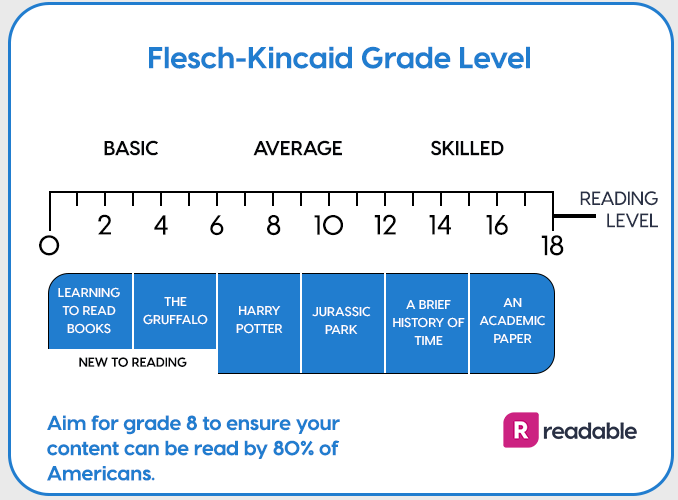
\includegraphics[width=\linewidth]{img/Screenshot_302.png}
	\caption{Afbeelding van \autocite{Readable2021}}
\end{figure}

% Bovendien zijn er kant-en-klare modellen die de complexiteit van tekst kunnen bepalen, hoewel deze beperkt zijn en vooral gericht zijn op Engelse teksten, zoals BERT\footnote{https://huggingface.co/docs/transformers/model\_doc/bert}, XLNet\footnote{https://huggingface.co/docs/transformers/model\_doc/xlnet}, GPT-3\footnote{https://platform.openai.com/docs/} en een open-source model genaamd TRUNAJOD\footnote{https://trunajod20.readthedocs.io/}.

%---------- Methodologie ------------------------------------------------------
\section{Methodologie}%
\label{sec:methodologie}

Het onderzoek houdt zes fases in. De eerste fase is het proces van tekstvereenvoudiging beschrijven, waaronder een omschrijving van het begrip en de verschillende soorten van technologische tekstvereenvoudiging. Dit gebeurt via een grondige studie van vakliteratuur en wetenschappelijke teksten. Ook blogs van experten komen hier aan bod. Na het verwerven van de nodige inzichten wordt er een verklarende tekst opgesteld.

De tweede fase bestaat uit het analyseren van wetenschappelijke werken over de bewezen voordelen van tekstvereenvoudiging bij scholieren met dyslexie van het derde graad middelbaar onderwijs. Hiervoor zijn geringe thesissen beschikbaar, die zorgvuldigheid vragen tijdens interpretatie. De resulterende tekst bevat de voordelen samen met hun wetenschappelijke onderbouwing.

De derde fase is opnieuw een beschrijving. Hier worden de valkuilen bij taalverwerking met AI-software nagegaan. Deze fase van het onderzoek brengt mogelijke nadelen en tekortkomingen van AI-software bij tekstvereenvoudiging aan het licht. Dit gebeurt aan de hand van een technische uitleg.

De vierde fase omvat een toelichting en advies over beschikbare AI-toepassingen voor tekstvereenvoudiging. Aan de hand van een veldonderzoek op het internet en bij bedrijven wordt er op zoek gegaan naar dergelijke software. Er wordt niet gezocht naar vertaalsoftware of toepassingen die de inhoud van een afbeelding of tekstbestand omzet naar tekstinhoud. Het resultaat is een shortlist van alle evaluatiecriteria waaraan de uitvoertekst van een tekstvereenvoudigingstoepassing moet voldoen.

De vijfde fase omschrijft de technische uitwerking van een pipeline voor tekstvereenvoudiging, alsook een shortlist van metrieken om de vereenvoudigde tekstinhoud te evalueren. Er zal een tekstvereenvoudigingspipeline worden ontwikkeld met beschikbare kant-en-klare bibliotheken, \textit{transformers} en algoritmen. Het resultaat van deze fase is een pipeline opgebouwd in de programmeertaal Python. 

De zevende en laatste fase omvat een vergelijkende studie van de gevonden tekstvereenvoudigingstoepassingen, alsook de tekstvereenvoudigingspipeline. Wetenschappelijke papers, die in een derde graad middelbaar onderwijs worden gebruikt, dienen hier als invoertekst voor de evaluatie. De transformatie wordt met zowel objectieve als subjectieve metrieken beoordeeld. De subjectieve test gebeurt aan de hand van een \textit{survey} en een \textit{think-aloudtest}. De objectieve testen gebeuren op basis van de shortlist uit de derde fase en de shortlist van metrieken uit de zesde fase. Ten slotte volgt er een persoonlijk advies over de nodige ontwikkelingen in het vak op vlak van Nederlandstalige tekstvereenvoudiging.

%---------- Verwachte resultaten ----------------------------------------------
\section{Verwacht resultaat, conclusie}
\label{sec:verwachte_resultaten}

Er wordt verwacht dat de software, die nu in het onderwijs wordt ingezet, niet voldoet aan de noden van een scholier met dyslexie in het derde graad middelbaar onderwijs. Dit is omdat er onvoldoende rekening wordt gehouden met hun unieke uitdagingen. Het vertalen van de uitvoertekst bij een internationale AI-toepassing zal vaak afwijken van de oorspronkelijke context. 

Er zijn onvoldoende kant-en-klare algoritmen en modellen beschikbaar om een pipeline voor tekstvereenvoudiging te bouwen. De vereenvoudigde inhoud uit de pipeline voldoet niet aan de unieke noden van een scholier met dyslexie in het derde graad middelbaar onderwijs. De pipeline vergt \textit{custom transformers} om belovende resultaten te bekomen. Het vertalen van de zinnen verlaagt de nauwkeurigheid van het model, maar het is een aanvaardbaar alternatief. Er is nood aan Nederlandstalige \textit{word embeddings} die de complexiteit per woord bijhouden, alsook meer kant-en-klare modellen die tekstsimplificatiefuncties aanbieden.